\section{Hashing Algorithm}
The term SHA (Secure Hash Algorithm) refers to a family of five different cryptographic hash functions developed since 1993 by the National Security Agency (NSA) and published by NIST as a federal standard by the U.S. government (FIPS PUB 180-4).

Like any hash algorithm, SHA produces a fixed-length message digest, or "message fingerprint," from a variable-length message. The security of a hash algorithm lies in the fact that the function is not invertible (i.e., it is not possible to find the original message knowing only this data) and that it must never be possible to intentionally create two different messages with the same digest. The algorithms of the family are named SHA-1, SHA-224, SHA-256, SHA-384 and SHA-512: the last 4 variants are often referred to generically as SHA-2, to distinguish them from the first one. The first one produces a message digest of only 160 bits, while the others produce digests of length in bits equal to the number indicated in their initials (SHA-256 produces a digest of 256 bits).

\begin{figure}[ht]
		\centering
		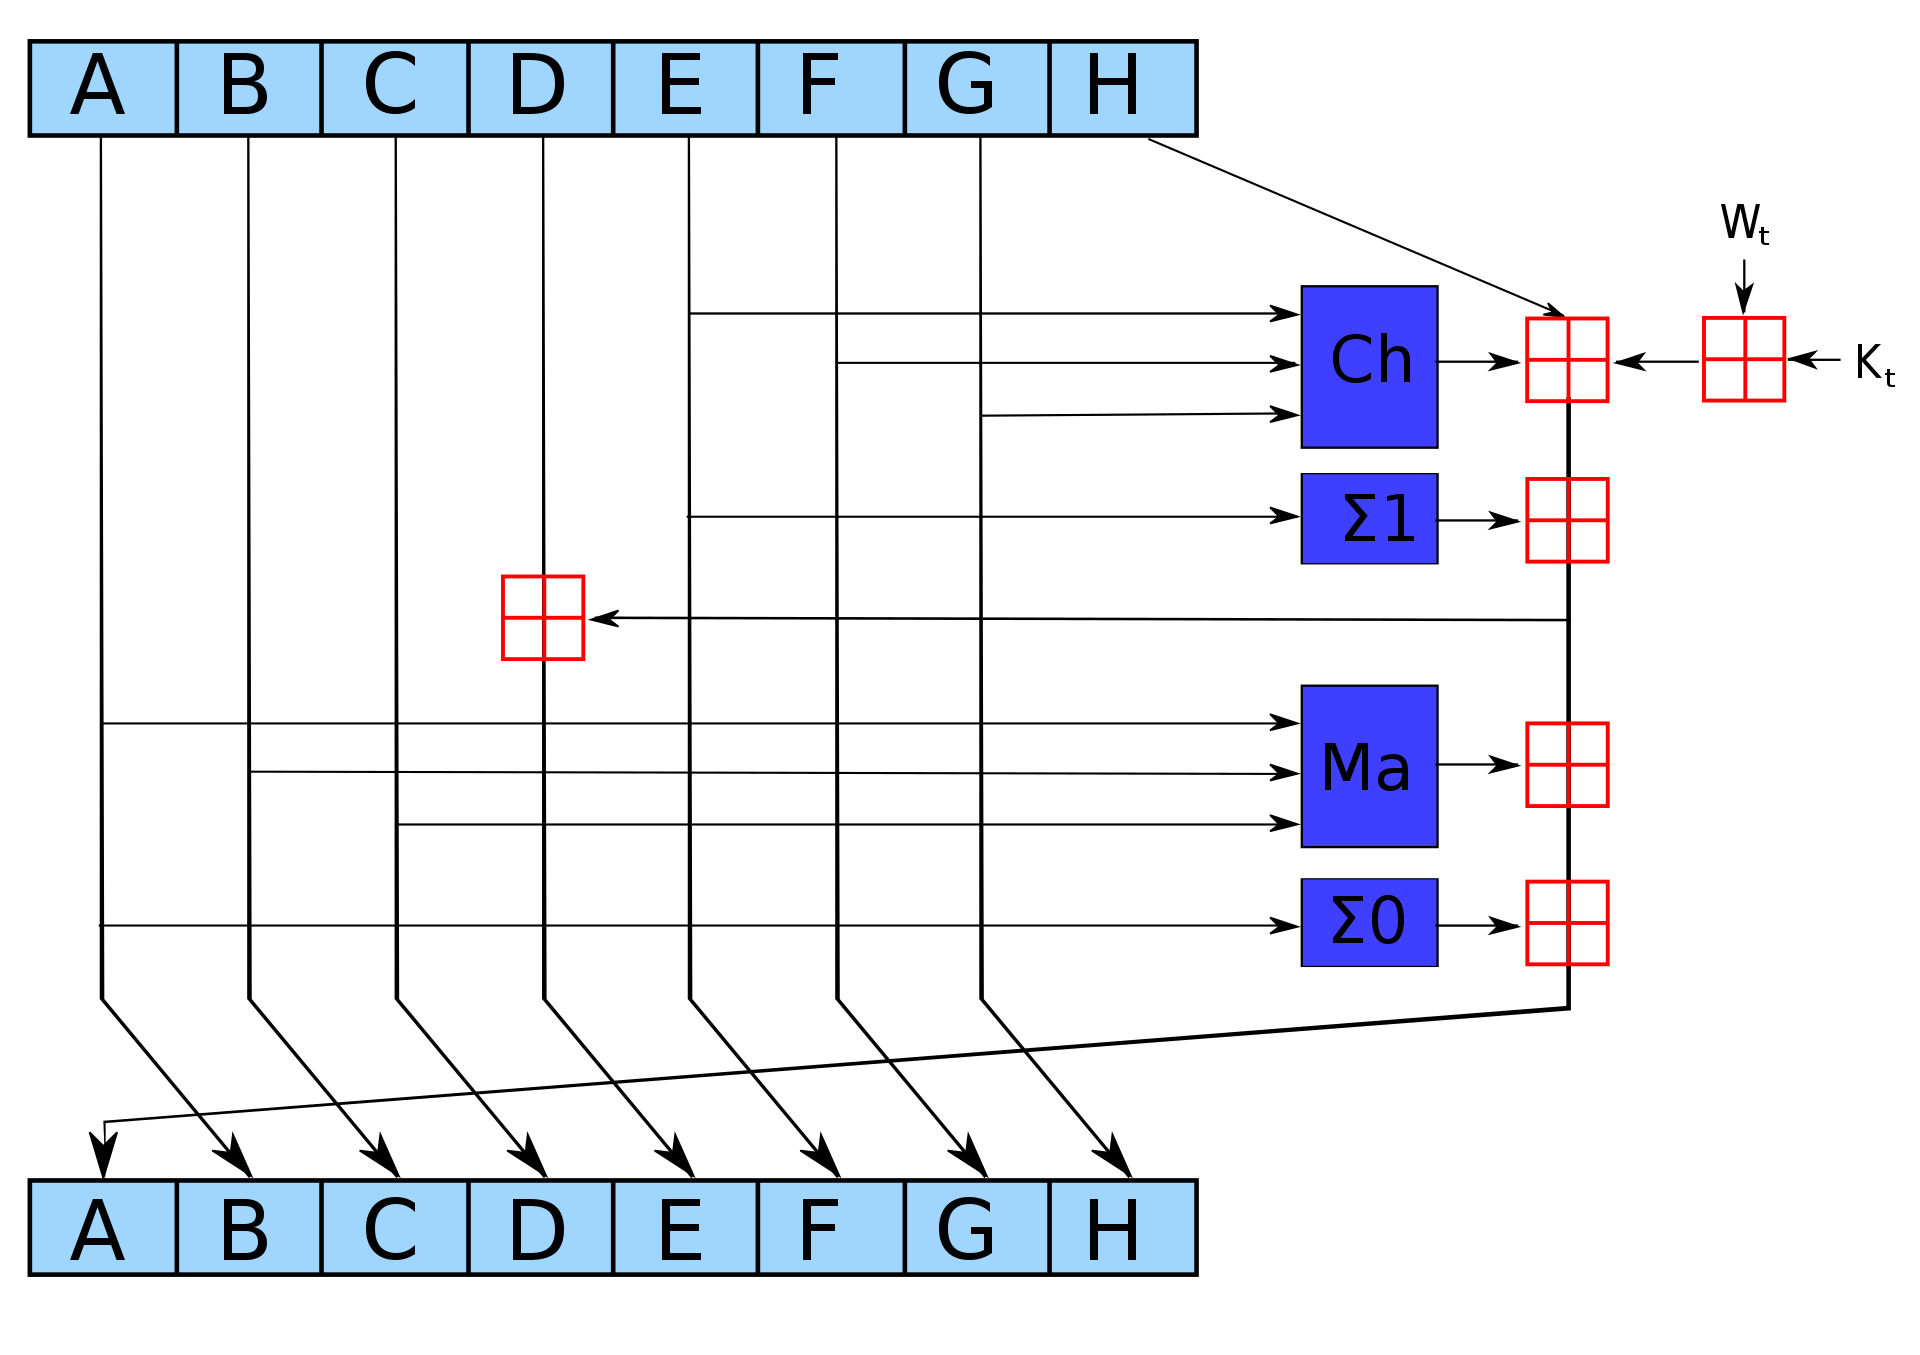
\includegraphics[width=.7\textwidth]{img/sha_iteration.png}
		\caption{Structure of a single SHA-2 iteration}
		\label{fig:sha_iteration}
\end{figure}

\autoref{fig:sha_iteration} shows the structure of an iteration of the SHA-256 algorithm. The main steps of the algorithm are the following:
\begin{enumerate}
	\item Initialize the variables and the table of round constants
	\item Pre-process the message
	\item Break the message in 512-bit chunks
	\item Extend the sixteen 32-bit words into sixty-four 32-bit words
	\item Initialize hash values
	\item Process the message (main loop)
	\item Produce the final hash value
\end{enumerate}